\documentclass[11pt]{article}
\usepackage[utf8]{inputenc}
\usepackage[T1]{fontenc}
\usepackage[francais]{babel}
\usepackage[francais]{layout}
\selectlanguage{french}

% NE PAS CHANGER !!
\ifx \public \undefined \def\public{etudiants} \fi
\usepackage[\public]{tps}

% Numéro du TP
\newcommand{\numtd}{05}
% Titre du TP
\newcommand{\titretd}{Codages de caractères}

\graphicspath{{imgs/}}

\begin{document}

\entete{\numtd}{\titretd}

\begin{introduction}
 Page web du cours :
 \begin{center}
  \url{http://www.lsv.ens-cachan.fr/~schwoon/enseignement/systemes/ws1718/}
 \end{center}

Le codage des caractères est une problématique censée être résolue par la
généralisation du codage de caractères UTF-8. Malheureusement, de nombreuses
applications anciennes et des machines mal configurées n'utilisent pas ce
standard par défaut.

La plupart des éditeurs de textes modernes, tel que vim, et des terminaux tel
que xfce4-terminal que vous utilisez actuellement permettent de choisir le
codage des caractères à utiliser pour l'édition des fichiers. 

La commande \textit{<<file>>} affiche les informations sur un fichier ainsi que
le mode d'encodage utilisé.

\end{introduction}

% {{{ Codage des caractères en HTML

\section{Codage des caractères en HTML}

Les pages HTML disposent de plusieurs façons de coder des caractères :\\

\begin{itemize}
 \item Les \emph{références d'entités} qui permettent de décrire
des caractères non-ASCII par des caractères ASCII, et ça indépendemment du
codage utilisé dans le reste du fichier. Ex. : \emph{à} s'écrit
\texttt{\&agrave;} dans cette notation.\smallskip
 \item Les \emph{références
numériques} qui donnent le code d'un caractère Unicode, sous la forme
\texttt{\&\#}\emph{nnn}\texttt{;} (décimal) ou
\texttt{\&\#x}\emph{nnn}\texttt{;}.\smallskip
 \item Le codage direct binaire
dans l'un des formats évoqué dans le cours (UTF-8, ISO-8859-1, \ldots). Ceci
nécéssite d'ajouter une balise de la forme :
 \begin{quote}
  \texttt{<meta http-equiv="Content-Type" content="text/html; charset=iso-8859-1" />}
 \end{quote}
dans le \texttt{header} du document HTML.\\
\end{itemize}

On va considérer les noms des communes européennes suivantes :
 \begin{quote}
 Crèvec\oe{}ur (France)\\ L'Ha\"y-les-Roses (France)\\ Krom\v{e}\v{r}\'i\v{z}
(Tchéquie)\\ G\"od\"oll\H{o} (Hongrie)\\ S\"u\ss{}en (Allemagne)\\
Pr\ae{}st\o{} (Danemark)
 \end{quote}

\begin{enumerate}
 \item Créez un document HTML qui affiche ces noms avec leurs
références d'entités.\smallskip
 \item Cherchez les codes Unicode des caractères
non-ASCII et utilisez-les pour recréer la liste avec des références
numériques.\smallskip
 \item Créez un document HTML en UTF-8 directement avec
votre éditeur de texte.
\end{enumerate}

% }}}

% {{{ Analyser une erreur de codage

\section{Analyser une erreur de codage}

Un grand classique que vous rencontrerez dans votre vie numérique est l'erreur
de codage sur des pages web. Vos connaissances actuelles couplées à ce que vous
avez vu en cours vous permettent de diagnostiquer \textbf{très précisément} le
type de dysfonctionnement auquel vous êtes confrontés.\bigskip

\subsection{Dans les pages html}

Rendez-vous à l'url suivante : \url{http://www.lsv.fr/~fhh/tp05-1}\bigskip

Décrivez et détaillez ce qui se passe en utilisant les tables de caratères
disponibles sur internet
(\url{https://fr.wikipedia.org/wiki/Table_des_caractères_Unicode_(0000-0FFF)}).
Proposez deux solutions permettant de corriger ce problème.

\begin{solution}

Nous sommes face à un problème d'encodage. Les caractères spéciaux s'affichent
sur deux ou trois caractères au lieu d'un. Il semble que nous soyons face à une
page UTF-8 interprétée en ISO8859-1.

\begin{itemize}
 \item é : à = 00c3 soit 11000011 ; © = 00a8 soit 10101000
 \item ç :
 \item Ã\"{ } : 
\end{itemize}

\end{solution}

\subsection{Erreur d'affichage SNCF}

En introduction au cours, nous vous avons montré l'erreur d'affichage relevée
sur un écran de la SNCF et présentée ci-dessous : 

\begin{center}
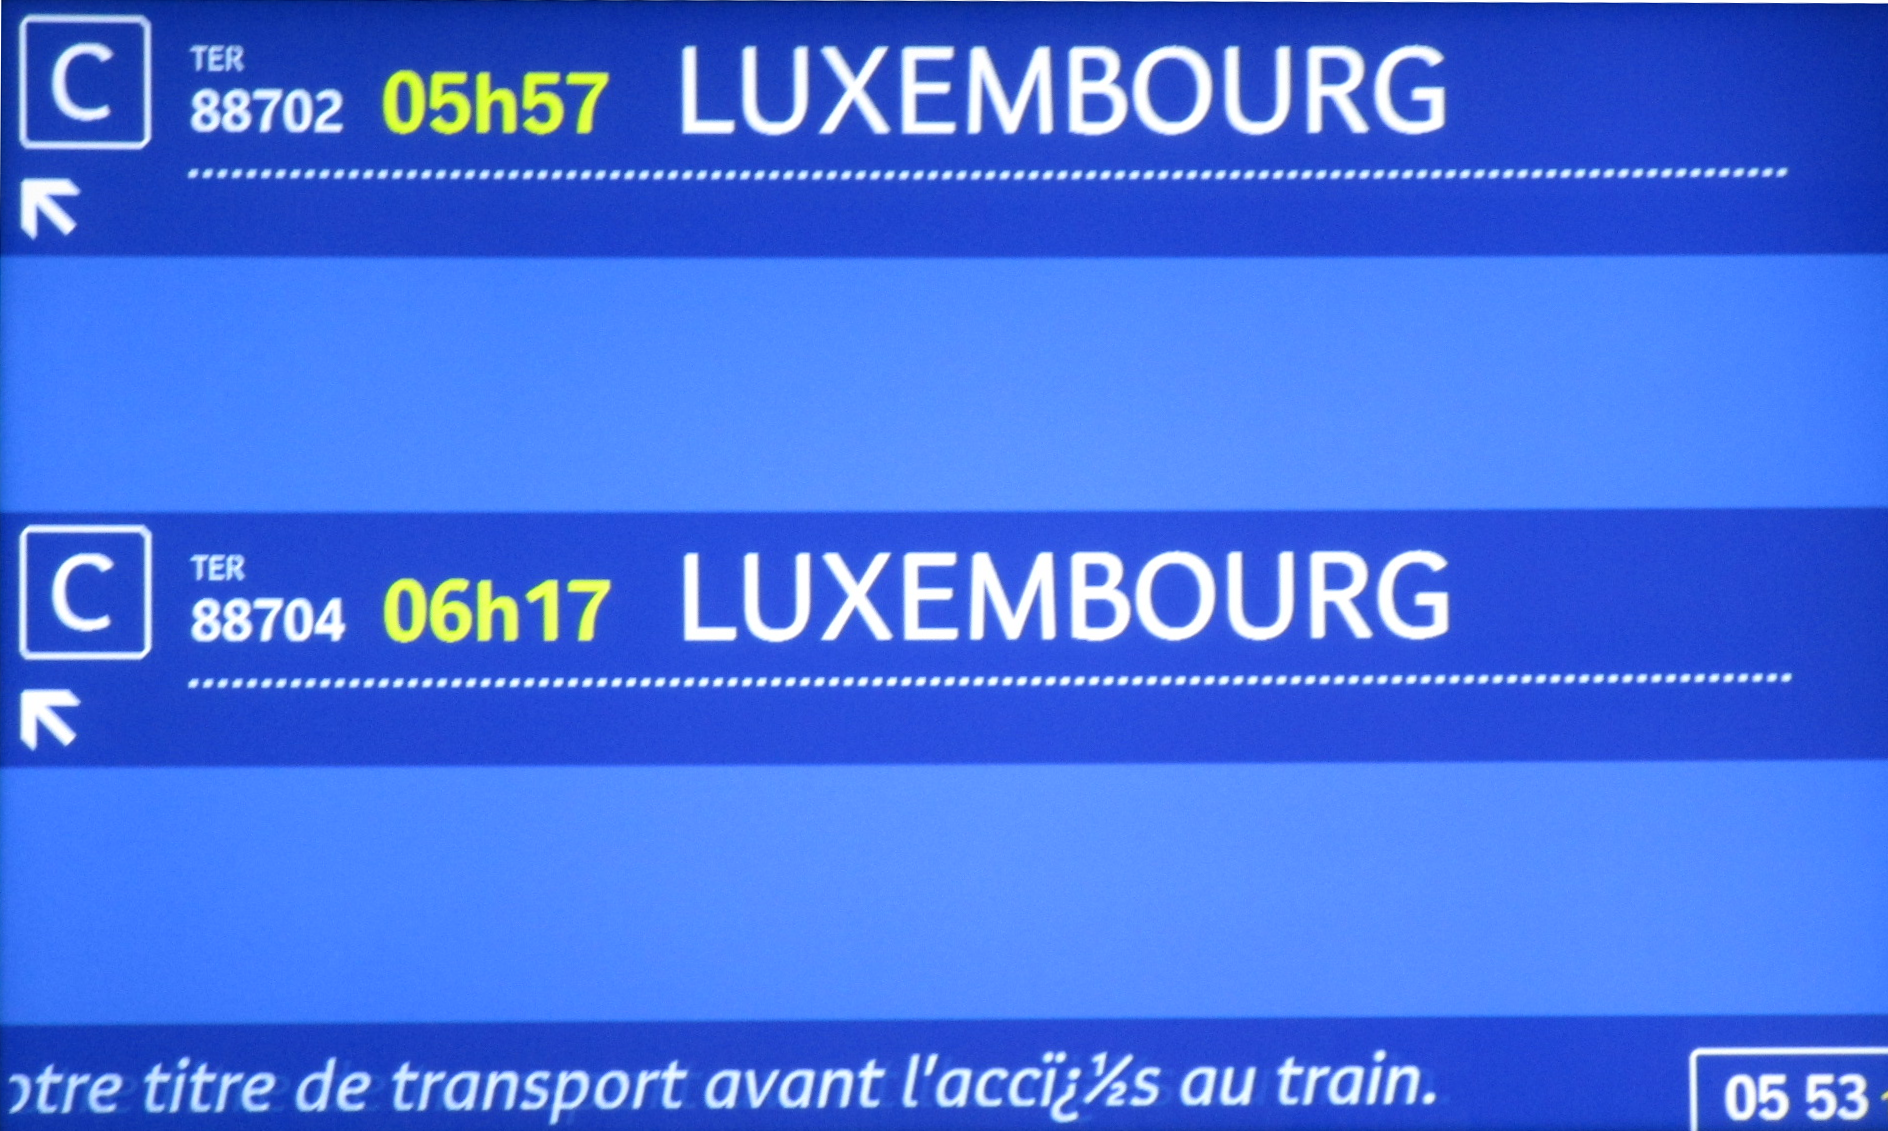
\includegraphics[width=10cm]{gare.png}
\end{center}

Observez attentivement ce bug d'affichage et déterminez ce qui s'est produit.

\subsection{Problème d'encodage de fichiers}

Téléchargez le fichier texte \url{http://www.lsv.fr/~fhh/tp05-2.txt} et affichez le dans votre navigateur.

Recherchez avec Firefox et Chrome les <<é>>.

Recherchez dans le fichier téléchargé les <<é>> avec la commande <<grep>>.

Que ce passe-t-il ? 

Proposez une solution permettant de corriger ce type de problème.

\begin{solution}
Les <<é>> sont codés de deux manière différentes. <<hexdump -C>> donne les codages des caractères.

Solution utiliser uconv -x NFD avant de mettre ce type de fichier dans une base de donnée.
\end{solution}

% }}}

% {{{ Configuration du clavier

\section{Configuration de votre clavier}

Vous pouvez ajouter des accès aux caractères exotiques tels que le caractère
néerlandais <<IJ>> ou <<ij>> à votre <<keymap>>. 

Proposez une solution pour que la combinaison de touche <<AltGr + i>> retourne
<<ij>> et <<AltGr + Shift + i>> retourne <<IJ>>.

% }}}

% {{{ Codage de caractères

\section{SMTP et Codage de caractères}

\subsection{Découverte du protocole}

Nous allons illustrer le problème d'encodage au travers de l'utilisation du
protocole SMTP définissant les règles d'acheminement des courriels et de la
commande <<telnet>> qui permet d'établir une connexion sur un port donné.

Le protocole SMTP (Simple Mail Transfer Protocol) est ancien et très simple :
\begin{itemize}

 \item une fois un client connecté sur un programme proposant la fonctionnalité
SMTP, le serveur répond avec le code 220 s'il accepte l'établissement de la
connexion ; 

 \item le client se présente via l'instruction <<HELO>> suivit de son nom. Le
serveur valide cette étape par un code 250 ;

 \item le client présente alors l'adresse de l'expéditeur du courriel précédé
de l'instruction <<MAIL FROM: >> auquel le serveur répond une nouvelle fois par
un code 250 (attention, le domaine d'expédition doit exister) ; 

 \item puis l'adresse du destinataire précédé de l'instruction <<RCPT TO: >>
validée par le serveur par un code 250 ; 

\item l'instruction <<DATA>> marque le début du contenu du message qui se
terminera par une ligne ne contenant qu'un point (<<.>>) ;

\item la connexion se termine via l'instruction <<QUIT>>.

\end{itemize}

Assurez-vous que le terminal que vous utilisez est configuré pour l'UTF-8,
envoyez un courriel à votre adresse puis renouveler l'opération avec un
terminal configuré en ISO-8859-1. Observez le résultat et commentez.

\subsection{Scripts d'envois de courriels}

Dans la séquence précédente, nous vous proposions d'utiliser la commande
<<telnet>> pour envoyer des courriels directement en contactant le serveur SMTP
de votre provider. Si vous tester ce procédé depuis l'extérieure, vous serez
confrontés à deux problèmes principaux :\\

\begin{itemize}
 \item Le serveur SMTP refuse la connexion : ce problème est dû
au fait que vous n'utilisiez pas le bon serveur SMTP. En effet, \textbf{vous
devez utiliser le serveur SMTP de votre provider}. Pour des raisons évidentes
de sécurité, vous ne pouvez pas utiliser, sans authentification, le serveur de
mail sortant d'Orange si vous êtes connecté à internet via un autre
prestataire. Vous ne pouvez pas plus utiliser le serveur SMTP de laposte.net
sans authentification.\\
 \item Le mail est refusé ou considéré comme SPAM :
pour lutter contre le SPAM, les providers contrôlent un certain nombre de
paramètres des mails tel que la présence d'un sujet. Les mails que vous envoyez
via <<telnet>> peuvent contenir ces <<headers>>, mais dans l'exemple proposé 
précédement, la modification des headers n'était pas spécifiée.\\
\end{itemize}

Une solution simple pour composer un courriel valide est d'utiliser un outil en
ligne de commande tel que <<s-nail>>, <<heirloom-mailx>>, etc, qui se chargera
de composer un courriel valide.\\

Sur les machines de la salle 411, l'outil installé est s-nail. Vous
pouvez consulter la page de manuel de l'outil pour découvrir les options
disponibles.\\

La première étape consiste à configurer s-nail dans le fichier
<<\textasciitilde{}/.mailrc>> pour qu'il utilise le serveur SMTP de votre
choix. Étudiez la configuration suivante et adaptez la à votre configuration
ENSC (serveur ENSPS en smtps, authentification plain) :

\begin{lstlisting} 
account gmail { 
 set smtp-use-starttls
 set ssl-verify=ignore
 set smtp-auth=login 
 set smtp=smtp://smtp.gmail.com:587
 set from="Jon Doe"
 set smtp-auth-user=jon.doe@gmail.com
 set smtp-auth-password=somePasword
}
\end{lstlisting}

\begin{solution} 
 \begin{lstlisting}
  account ensc {
   set ssl-verify=ignore
   set smtp-auth=plain
   set smtp=smtps://smtp.ens-paris-saclay.fr:465
   set from="Francis HULIN-HUBARD <fhh@votre domaine>"
   set smtp-auth-user=<login ensc>
   set smtp-auth-password=XXXXXXXXXXX
  }
 \end{lstlisting}
\end{solution}

Essayez votre configuration.

\begin{solution} date +\%s | mail -v -A ensc -s Paf2 fhh@lsv.fr \end{solution}

Créez un profil utilisant le serveur du département.

\begin{solution}
 \begin{lstlisting}
 account dpt {
  set smtp=smtp://mailhost.dptinfo.ens-cachan.fr 
 }
 \end{lstlisting}
\end{solution}

Proposez un profil utilisant un serveur Orange, OVH ou Free.\\

L'option <<-A>> permet de sélectionner le profil utilisé pour l'envoi d'un
courriel. 

\begin{lstlisting}
 mail -A gmail adresse@domain.tld
\end{lstlisting}

Envoyez un courriel en utilisant votre profil ENSC puis en utilisant le profil
de votre provider.\\

\begin{center} \textbf{<<Oui, mais du coup, les mails n'ont rien d'anonyme
!!>>} \end{center}

En effet, par défaut, les mails n'ont rien d'anonyme, mais en étudiant les
paramètres de la commande <<mail>>, vous verrez qu'il est possible de modifier
l'adresse de l'expéditeur du message.\\

Envoyez vous un courriel provenant de l'adresse <<jean.bon@lsv.fr>>.
Étudiez les entêtes du courriel.

\begin{solution}

Option '-r adresse expéditeur'

cat /import/fhh/.mailrc | mail -r "Jean BON <jean.bon@lsv.fr>" -s "Fichier de
configuration ~/.mailrc" fhh@lsv.fr

Entêtes :

\begin{verbatim} Return-Path: <fhh@e-galaxie.org> X-Original-To:
fhh@e-galaxie.org Delivered-To: fhh@e-galaxie.org X-Spam-Status: No
X-EGO-SI-From: fhh@e-galaxie.org X-EGO-SI-SpamCheck: n'est pas un polluriel,
SpamAssassin (score=-1.9, requis 6, autolearn=not spam, BAYES_00 -1.90,
RCVD_IN_DNSWL_NONE -0.00) X-EGO-SI: Found to be clean X-EGO-SI-ID:
6BC656571.AD9A3 X-EGO-SI-Information: To informations about mails traitments
contact your service informatique Received: from olive.lsv.ens-cachan.fr
(olive.lsv.fr [138.231.81.248]) by mail.e-galaxie.org (Postfix) with ESMTP id
6BC656571 for <fhh@e-galaxie.org>; Thu, 20 Oct 2016 14:36:40 +0200 (CEST)
Received: by olive.lsv.ens-cachan.fr (Postfix) id 29B9B4C01A9; Thu, 20 Oct 2016
14:36:40 +0200 (CEST) Delivered-To: fhh@lsv.fr Received: from
ariane2.ens-cachan.fr (ariane2.ens-cachan.fr [138.231.176.54]) by
olive.lsv.ens-cachan.fr (Postfix) with ESMTP id 281AC4C0186 for <fhh@lsv.fr>;
Thu, 20 Oct 2016 14:36:40 +0200 (CEST) Received: from localhost (localhost
[127.0.0.1]) by ariane2.ens-cachan.fr (Postfix) with ESMTP id 1B3FD142514 for
<fhh@lsv.fr>; Thu, 20 Oct 2016 14:36:39 +0200 (CEST) X-Virus-Scanned: Debian
amavisd-new at ens-cachan.fr Received: from ariane2.ens-cachan.fr ([127.0.0.1])
by localhost (ariane2.ens-cachan.fr [127.0.0.1]) (amavisd-new, port 10026) with
ESMTP id 3XBACuUWF_q7 for <fhh@lsv.fr>; Thu, 20 Oct 2016 14:36:39 +0200 (CEST)
Received: from 08.dptinfo.ens-cachan.fr (08.dptinfo.ens-cachan.fr
[138.231.36.108]) (using TLSv1.2 with cipher ECDHE-RSA-AES256-GCM-SHA384
(256/256 bits)) (No client certificate requested) by ariane2.ens-cachan.fr
(Postfix) with ESMTPSA id BADA7142509 for <fhh@lsv.fr>; Thu, 20 Oct 2016
14:36:39 +0200 (CEST) Date: Thu, 20 Oct 2016 14:36:38 +0200 From: Francis
HULIN-HUBARD <fhh@e-galaxie.org> To: fhh@lsv.fr Subject: Paf Message-ID:
<5808ba56./RUcSgsYhjKsCF+F%fhh@e-galaxie.org> User-Agent: Heirloom mailx 12.5
6/20/10 MIME-Version: 1.0 Content-Type: text/plain; charset=us-ascii
Content-Transfer-Encoding: 7bit X-Greylist: Sender IP whitelisted, not delayed
by milter-greylist-4.3.7 (mail.e-galaxie.org [0.0.0.0]); Thu, 20 Oct 2016
14:36:40 +0200 (CEST)

1476966998 \end{verbatim} \end{solution}

% }}}

\end{document}
